\renewcommand{\baselinestretch}{1.5}

\chapter{CONCEPTOS DE SOLUCIÓN}

\section{Concepto de solución 1}

El primer concepto de solución agrupa tecnologías económicas ideales para validaciones académicas, pruebas de concepto iniciales o entornos controlados. Estructuralmente, los componentes se protegen dentro de una carcasa fabricada íntegramente en MDF, y su movilidad recae en cuatro ruedas omnidireccionales, aptas para superficies planas, aunque limitadas en campo abierto. Para el despliegue de sus instrumentos climáticos, cuenta con sensores meteorológicos fijos sobre la cubierta y utiliza una plataforma de medición elevable, impulsada por un motor DC y un mecanismo de piñón y cremallera, sobre la cual se aloja un sensor de irradiancia. En el apartado de energía e interfaz, el sistema recibe alimentación a través de conectores Plug Jack y un selector rotativo que dirigen la energía hacia reguladores de voltaje y un Battery Management System acoplado a una batería NiMh. La interfaz física exterior incluye conectores roscados, un panel de luces LED de colores para indicaciones visuales y emite alertas simples a través de un buzzer. Su percepción y navegación se apoyan físicamente en un módulo GPS interno, complementado con el registro de datos en un módulo de memoria FLASH. Finalmente, el control y la lógica se centralizan en un microcontrolador que, a nivel de software, procesa datos mediante tablas de búsqueda, usa control SMC, guía el vehículo mediante el controlador Stanley paralelo y evade obstáculos comparando umbrales temporales.

\begin{figure}[H]
	% Fuerza la alineación izquierda y quita los ":" después del número
	\captionsetup{justification=raggedright, singlelinecheck=false, labelsep=none}
	
	\caption[Diseño general de la solución 1.]{} 
	
	% Vspace negativo opcional para acercar el texto cursivo al número de figura
	\textit{Diseño general de la solución 1.} \par\medskip
	
	\centering
	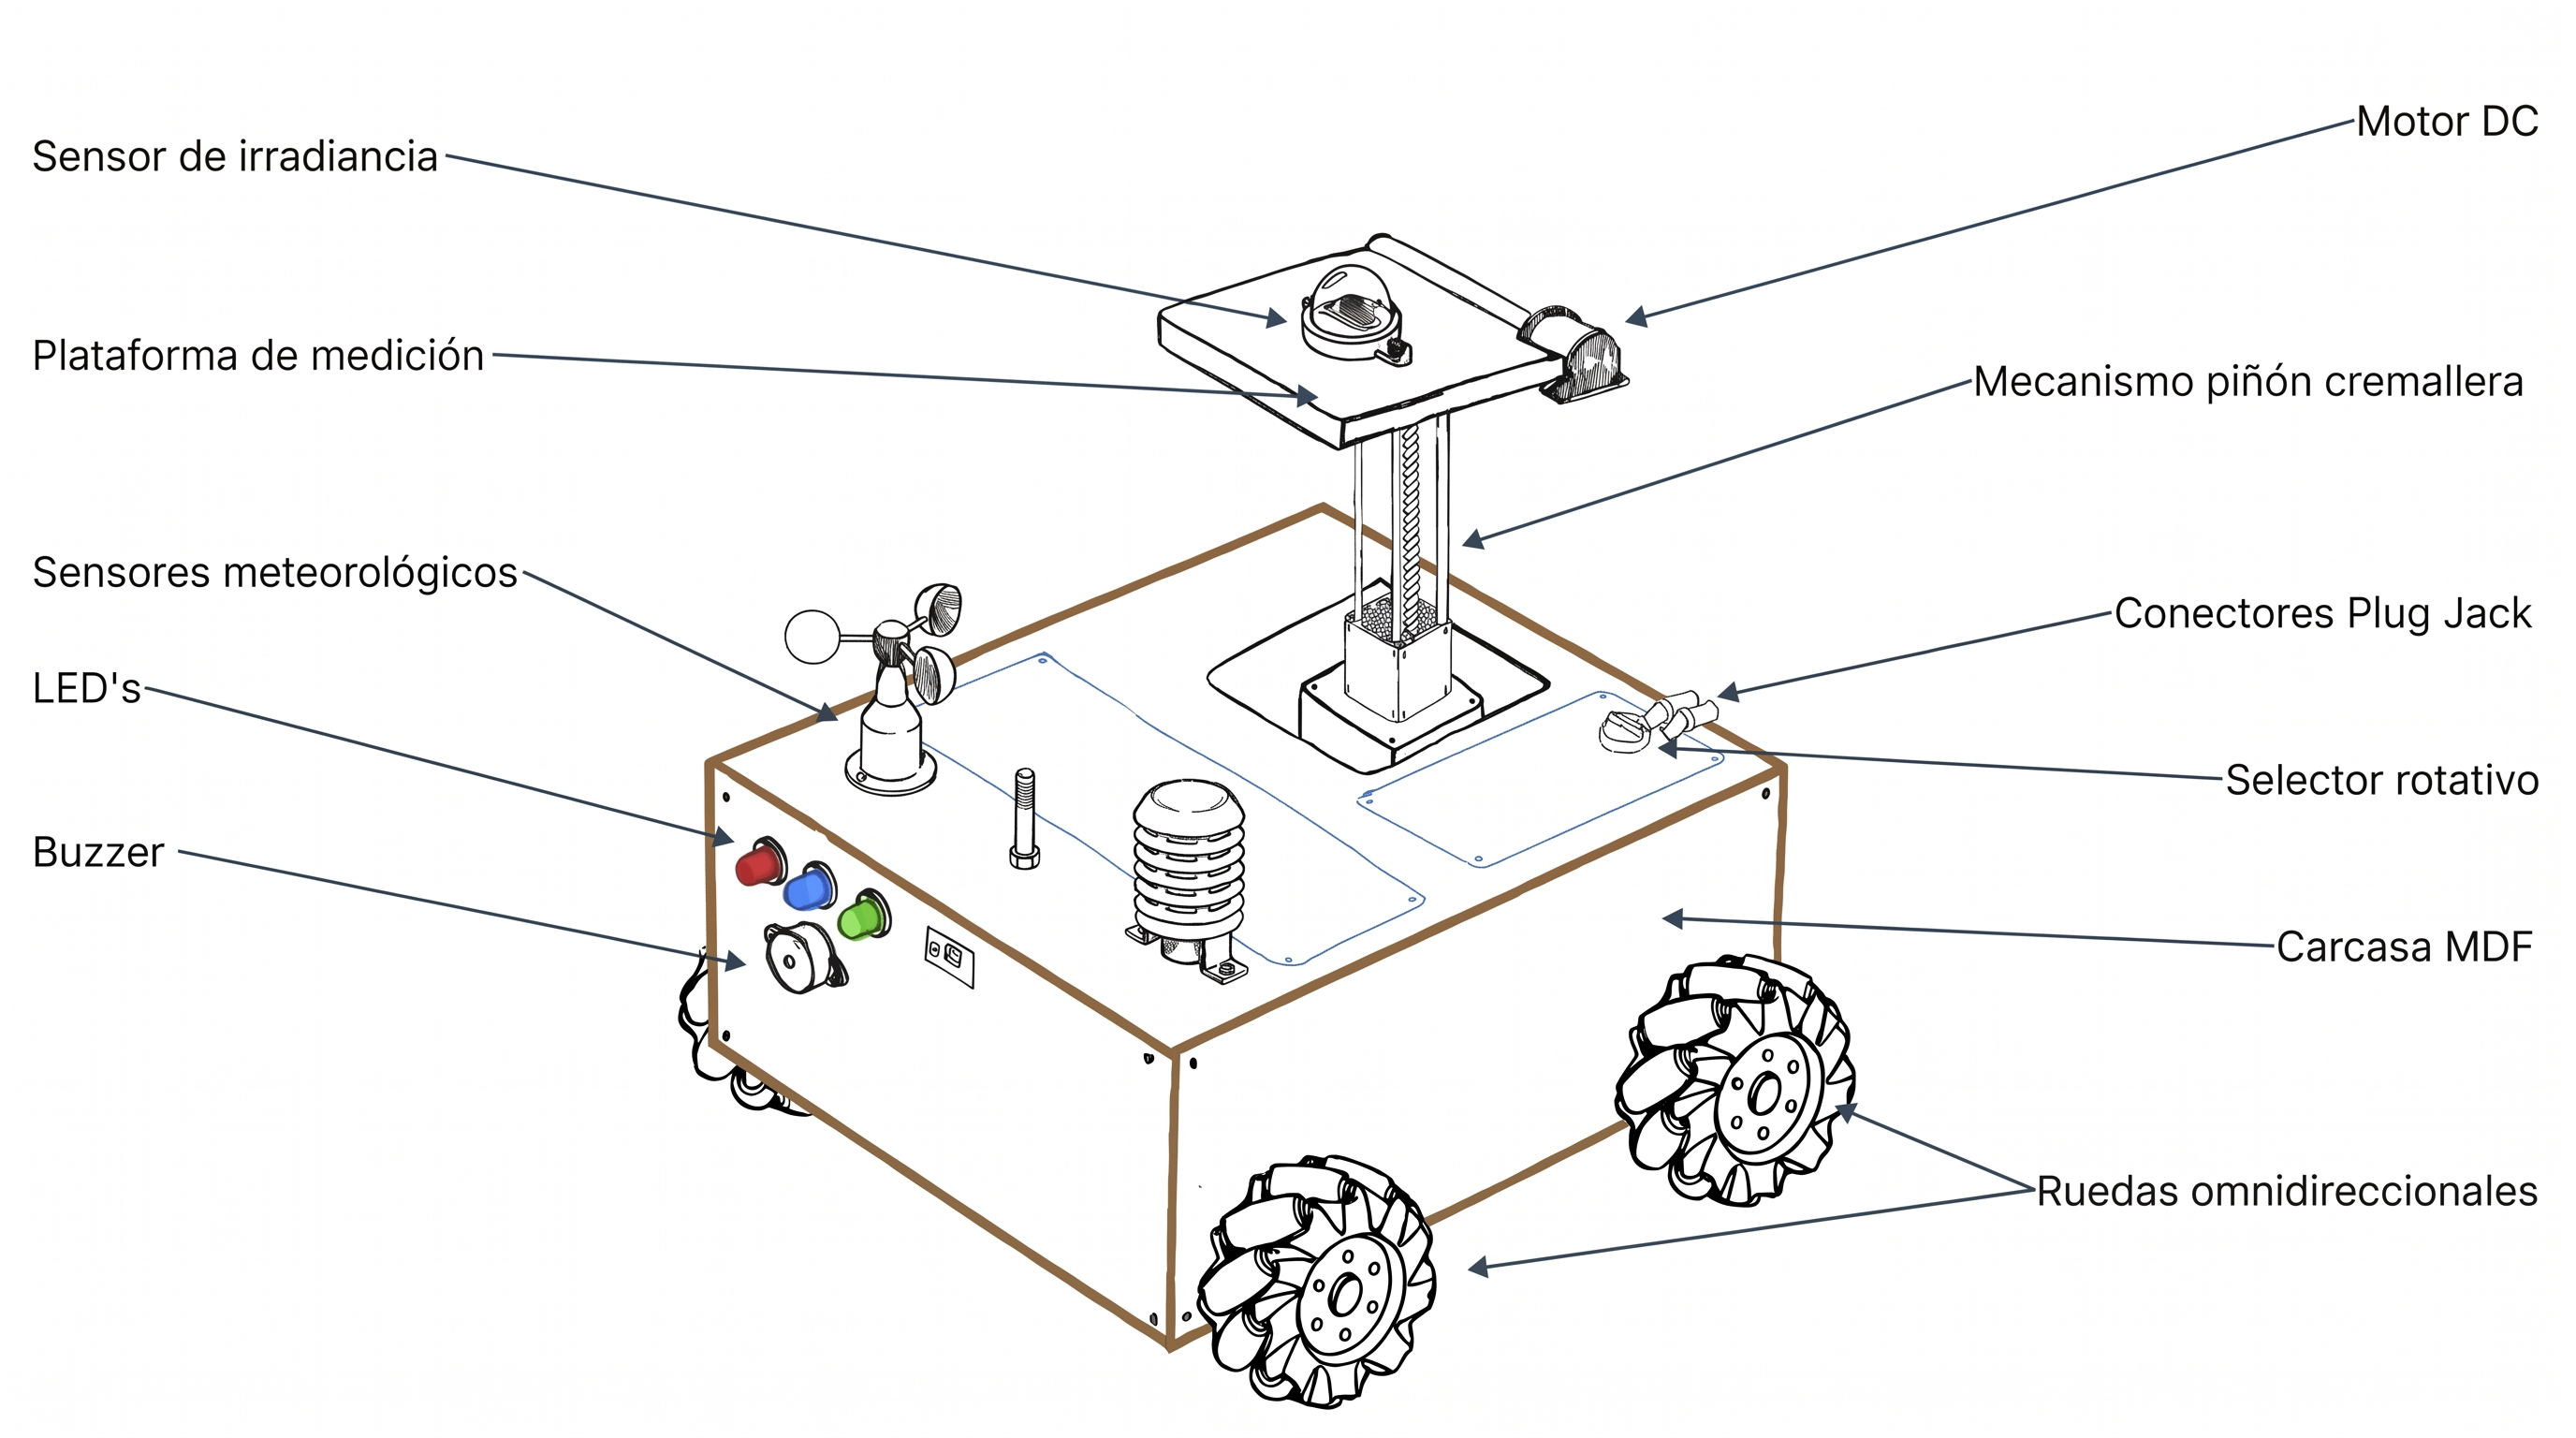
\includegraphics[width=\textwidth]{ImagenesConceptos/A-General.jpeg} \par\medskip
	
	\raggedright
	\footnotesize \textit{Nota.} Elaboración propia, asistida con IA generativa.
	\label{fig:AGeneral}
\end{figure}

\begin{figure}[H]
	% Fuerza la alineación izquierda y quita los ":" después del número
	\captionsetup{justification=raggedright, singlelinecheck=false, labelsep=none}
	
	\caption[Diseño interno de la solución 1.]{} 
	
	% Vspace negativo opcional para acercar el texto cursivo al número de figura
	\textit{Diseño interno de la solución 1.} \par\medskip
	
	\centering
	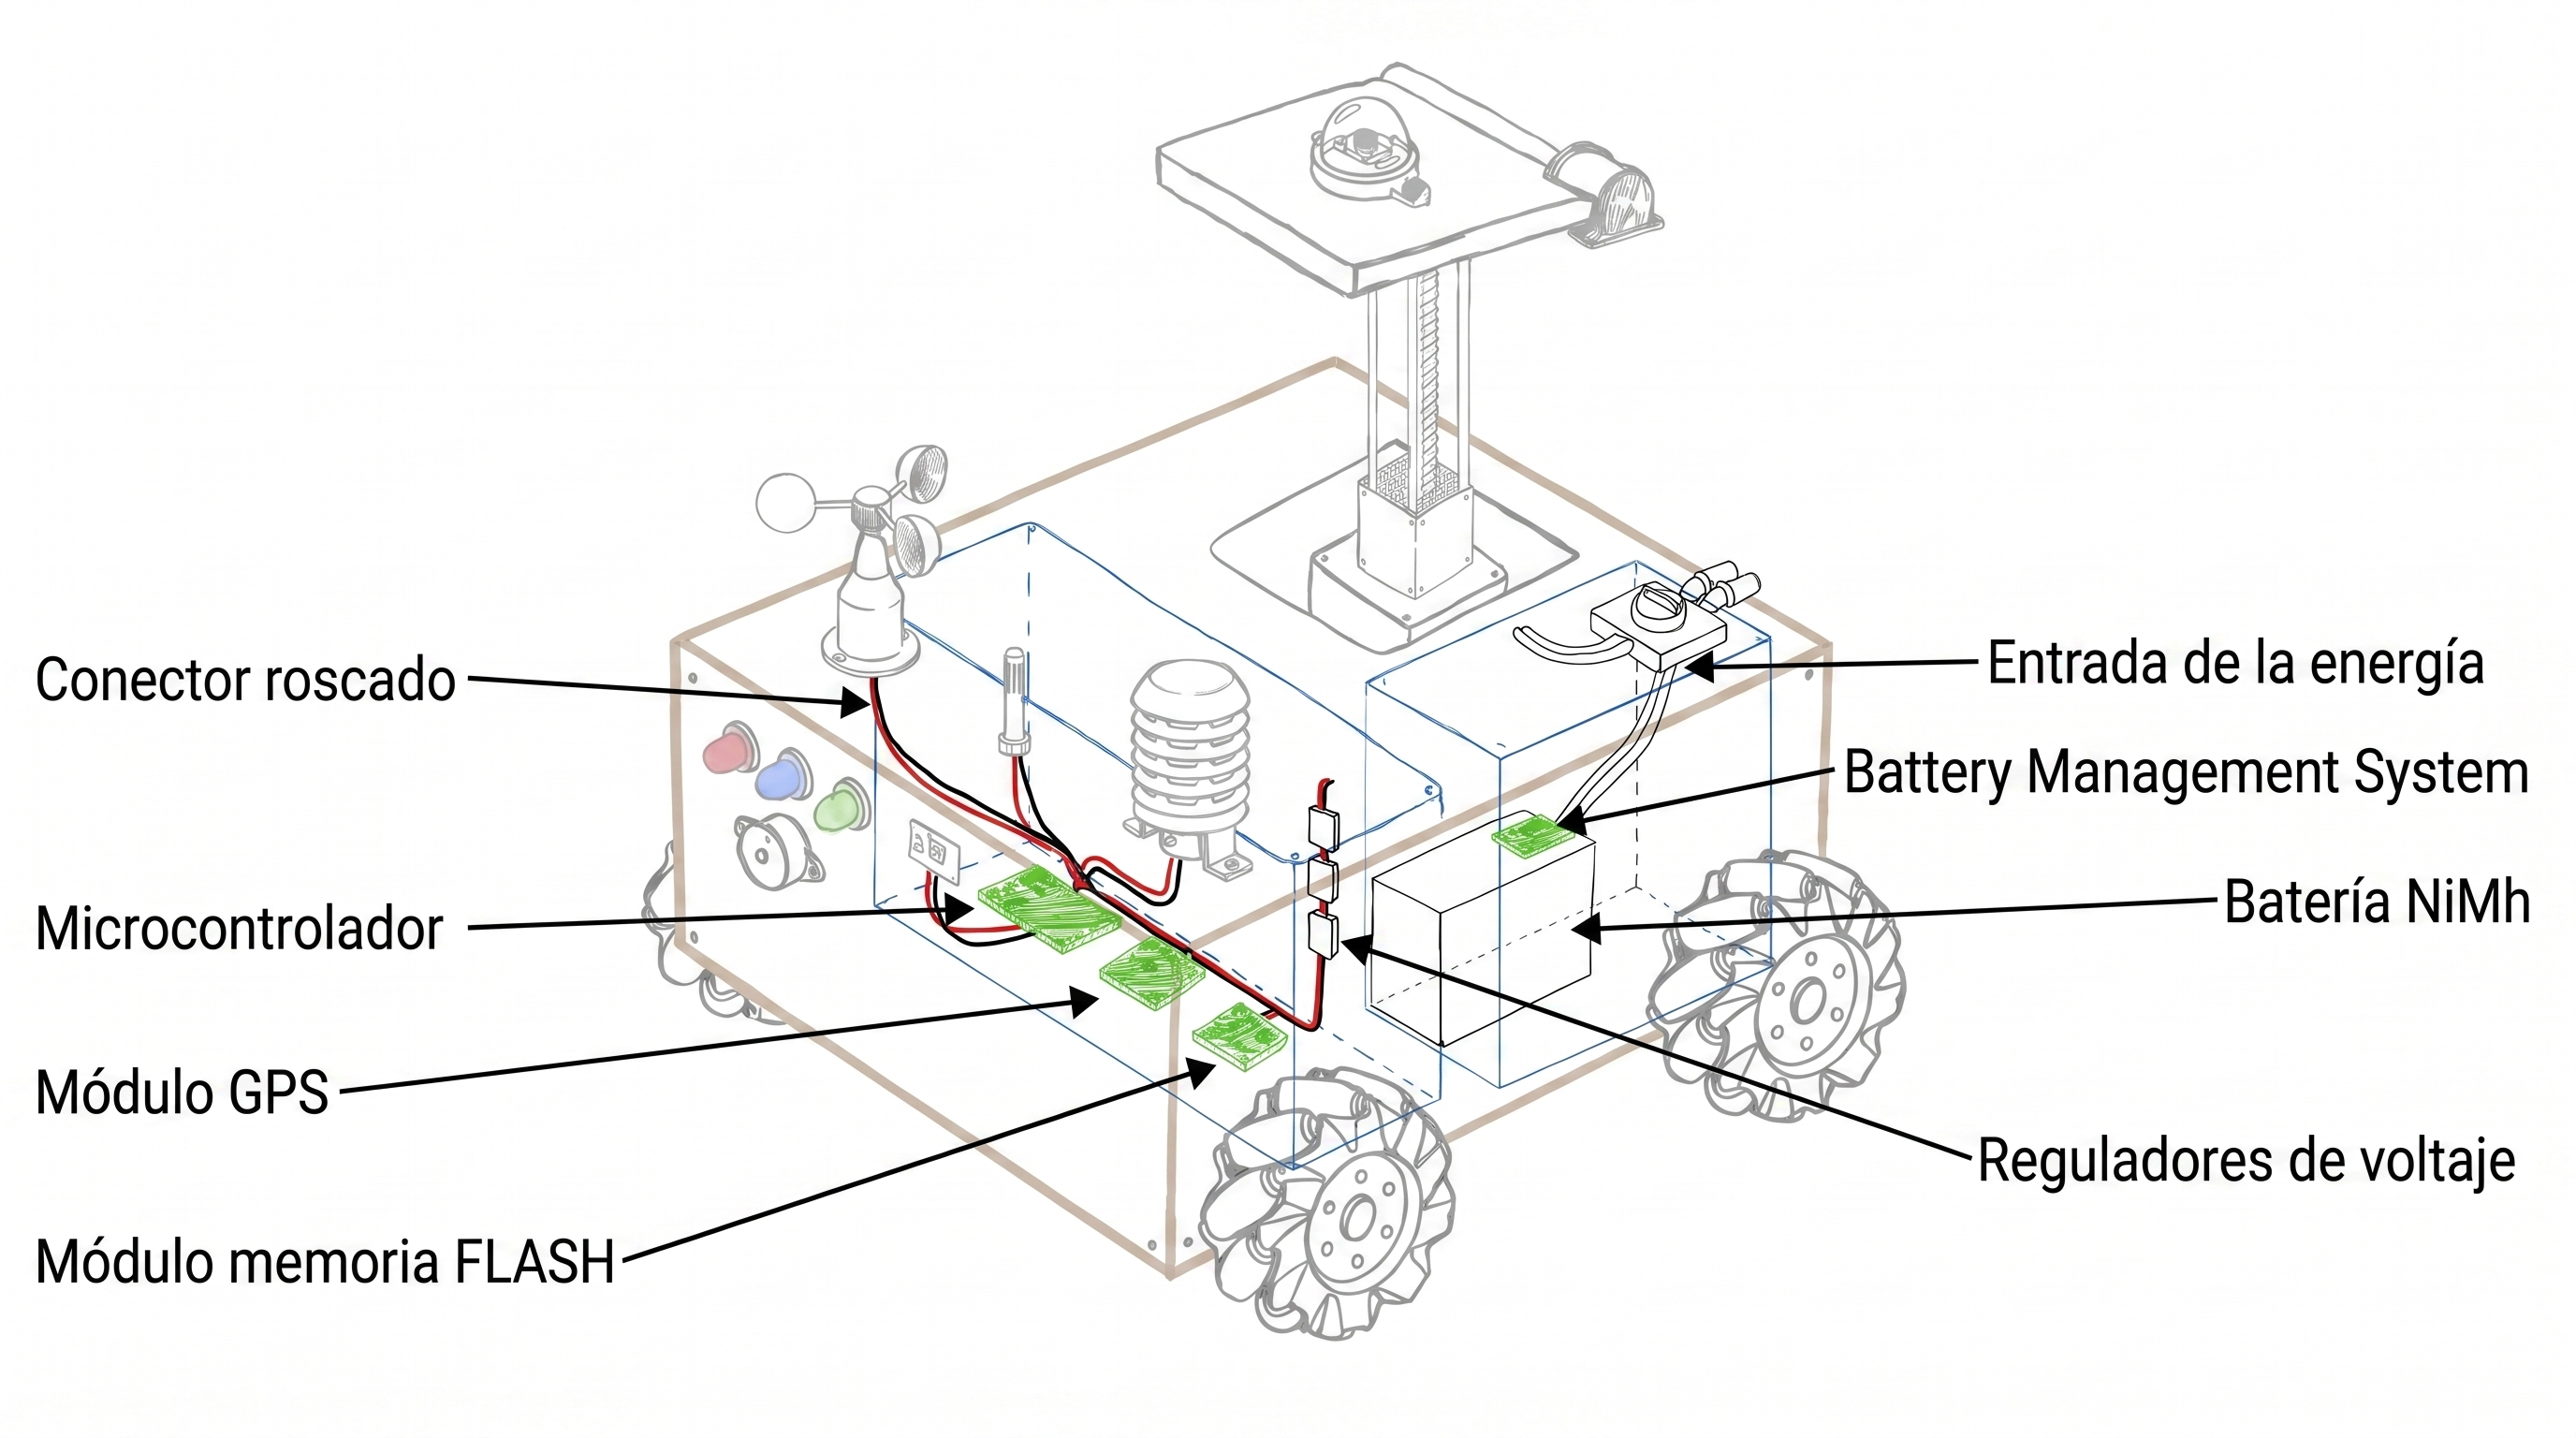
\includegraphics[width=\textwidth]{ImagenesConceptos/A-Interno.jpeg} \par\medskip
	
	\raggedright
	\footnotesize \textit{Nota.} Elaboración propia, asistida con IA generativa.
	\label{fig:AInterno}
\end{figure}

\section{Concepto de solución 2}

Este concepto representa un equilibrio óptimo entre robustez técnica, costo y capacidad de procesamiento para entornos de parques solares. A nivel mecánico y estructural, el equipo está construido sólidamente con una carcasa de aluminio y su desplazamiento se da por tracción diferencial mediante cuatro ruedas. Además, cuenta con una plataforma superior de instrumentación móvil que asegura gran precisión e inamovilidad gracias al uso de mecanismos de tornillo sin-fin y corona accionados por un servomotor DC. En cuanto a energía e interfaz, el robot presenta una alta confiabilidad operando con una batería de iones de litio protegida por sistemas de gestión de batería y reguladores de voltaje internos. Su interfaz exterior emplea borneras industriales para sus conexiones y cuenta con una pantalla LCD junto a una pantalla HMI lateral para interactuar e informar sobre su estado. Para la percepción y exploración, el sistema adquiere datos del entorno mediante sensores meteorológicos y un sensor de irradiancia ubicados en su plataforma elevadiza, emplea un módulo CMOS frontal para la visión por cámara, y transmite o recibe telemetría a través de una antena externa. Finalmente, en cuanto a control y lógica, el cerebro central del robot es una placa SBC que registra la información recopilada en un módulo de memoria microSD. Para ejecutar los cálculos complejos y procesar el video de la cámara, la SBC se apoya directamente en un Acelerador Edge IA, lo que le permite procesar el entorno de manera eficiente mientras utiliza control PID para los motores y traza su trayectoria con el Algoritmo Pure Pursuit.

\begin{figure}[H]
	% Fuerza la alineación izquierda y quita los ":" después del número
	\captionsetup{justification=raggedright, singlelinecheck=false, labelsep=none}
	
	\caption[Diseño general de la solución 2.]{} 
	
	% Vspace negativo opcional para acercar el texto cursivo al número de figura
	\textit{Diseño general de la solución 2.} \par\medskip
	
	\centering
	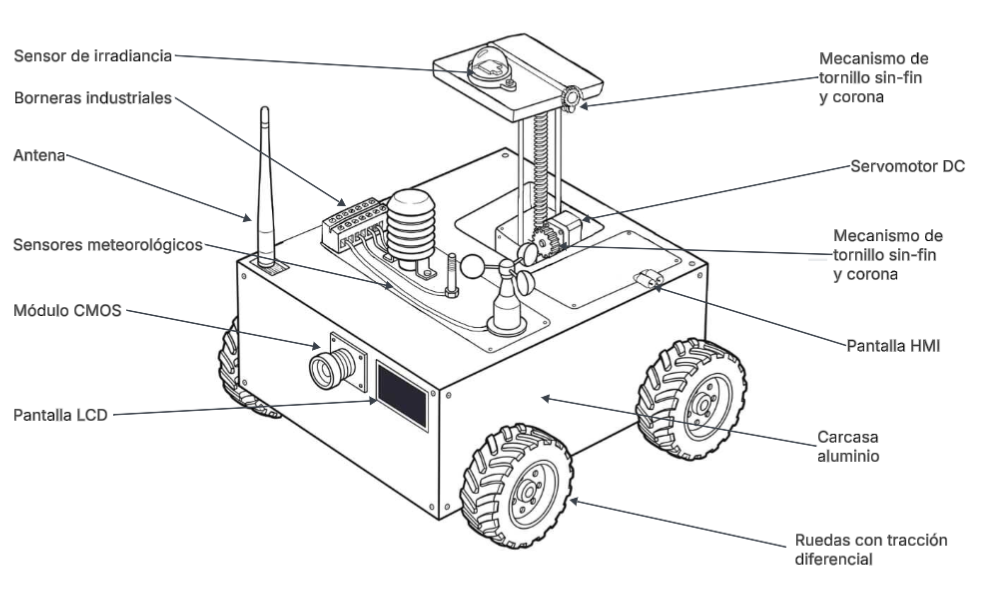
\includegraphics[width=\textwidth]{ImagenesConceptos/B-General.png} \par\medskip
	
	\raggedright
	\footnotesize \textit{Nota.} Elaboración propia, asistida con IA generativa.
	\label{fig:BGeneral}
\end{figure}

\begin{figure}[H]
	% Fuerza la alineación izquierda y quita los ":" después del número
	\captionsetup{justification=raggedright, singlelinecheck=false, labelsep=none}
	
	\caption[Diseño interno de la solución 2.]{} 
	
	% Vspace negativo opcional para acercar el texto cursivo al número de figura
	\textit{Diseño interno de la solución 2.} \par\medskip
	
	\centering
	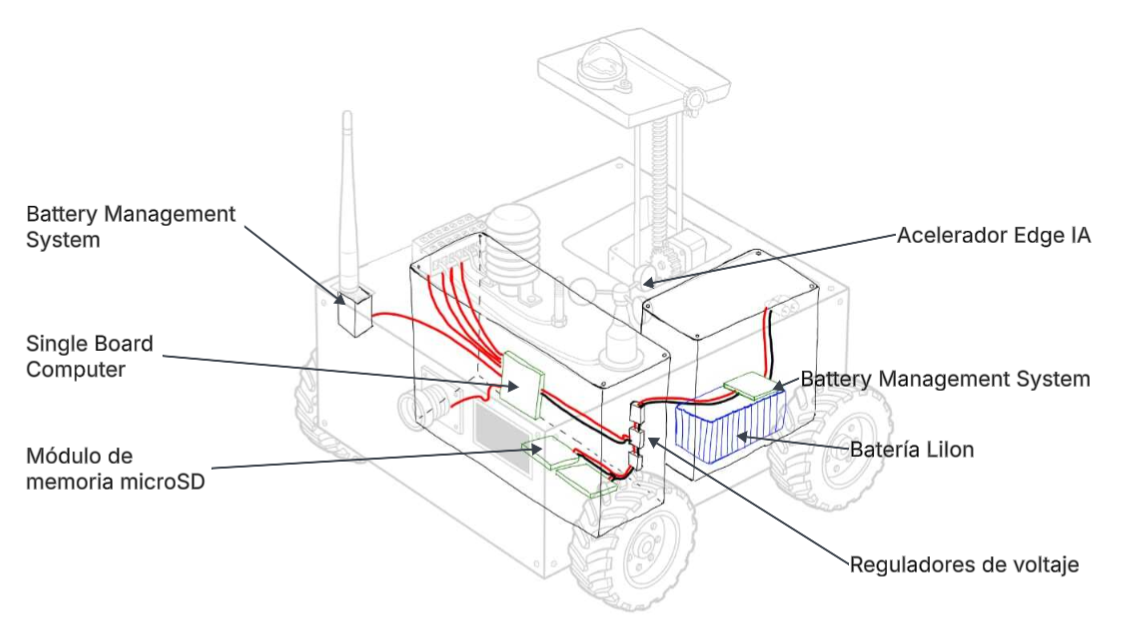
\includegraphics[width=\textwidth]{ImagenesConceptos/B-Interno.png} \par\medskip
	
	\raggedright
	\footnotesize \textit{Nota.} Elaboración propia, asistida con IA generativa.
	\label{fig:BInterno}
\end{figure}

\section{Concepto de solución 3}

El tercer concepto de soluciíon corresponde al nivel tecnológico industrial, diseñado para resistir las condiciones topográficas y climáticas más agresivas. Su estructura mecánica emplea un blindaje mediante una carcasa principal de acero y garantiza la movilidad en terrenos accidentados gracias a un sistema de ruedas con tracción de oruga que es impulsado internamente por un motorreductor DC. Además, el equipo integra una plataforma de medición que descansa sobre un actuador lineal vertical y opera mediante un motor DC acoplado a un mecanismo de correa dentada. En el apartado de energía e interfaz, el robot dispone de un sistema de carga exterior mediante contactos magnéticos, reguladores de voltaje internos y se alimenta con una batería LiPo protegida por un Battery Management System. Todo el cableado y la electrónica interna utilizan conexiones herméticas Deutsch, mientras que el chasis exterior se complementa con una pantalla HMI para la interacción directa y una sirena LED de señalización. La percepción y lectura del entorno están a cargo de un sensor LiDAR frontal, apoyado por sensores meteorológicos y un sensor de irradiancia montados en la plataforma superior. Finalmente, el control y la lógica del sistema son gobernados por un PLC, el cual trabaja en paralelo con un acelerador Edge IA para procesar eficientemente los datos del entorno, como la segmentación de nubes de puntos del LiDAR, permitiendo así una navegación avanzada.

\begin{figure}[H]
	% Fuerza la alineación izquierda y quita los ":" después del número
	\captionsetup{justification=raggedright, singlelinecheck=false, labelsep=none}
	
	\caption[Diseño general de la solución 3.]{} 
	
	% Vspace negativo opcional para acercar el texto cursivo al número de figura
	\textit{Diseño general de la solución 3.} \par\medskip
	
	\centering
	
\includegraphics[width=\textwidth]{ImagenesConceptos/C-General.png} \par\medskip
	
	\raggedright
	\footnotesize \textit{Nota.} Elaboración propia, asistida con IA generativa.
	\label{fig:CGeneral}
\end{figure}

\begin{figure}[H]
	% Fuerza la alineación izquierda y quita los ":" después del número
	\captionsetup{justification=raggedright, singlelinecheck=false, labelsep=none}
	
	\caption[Diseño interno de la solución 3.]{} 
	
	% Vspace negativo opcional para acercar el texto cursivo al número de figura
	\textit{Diseño interno de la solución 3.} \par\medskip
	
	\centering
	
\includegraphics[width=\textwidth]{ImagenesConceptos/C-Interno.png} \par\medskip
	
	\raggedright
	\footnotesize \textit{Nota.} Elaboración propia, asistida con IA generativa.
	\label{fig:CInterno}
\end{figure}

\section{Evaluación técnica}

\begin{table}[H]
	\captionsetup{justification=raggedright, singlelinecheck=false, labelsep=none}
	
	\caption[Matriz de Evaluación Técnica de Conceptos de Solución.]{} 
	\textit{Matriz de Evaluación Técnica de Conceptos de Solución.} \par\medskip
	
	\centering
	\footnotesize
	\renewcommand{\arraystretch}{1.3} 
	\begin{tabular}{|p{5.5cm}|c|c|c|c|c|c|c|c|c|}
		\hline
		\rowcolor[HTML]{D9E1F2} 
		\multirow{2}{*}{\textbf{Criterio de Evaluación}} & \multirow{2}{*}{\textbf{Peso (G)}} & \multicolumn{2}{c|}{\textbf{Solución 1}} & \multicolumn{2}{c|}{\textbf{Solución 2}} & \multicolumn{2}{c|}{\textbf{Solución 3}} & \multicolumn{2}{c|}{\textbf{Sol. Ideal}} \\ \cline{3-10}
		\rowcolor[HTML]{D9E1F2} 
		& & \textbf{P} & \textbf{GP} & \textbf{P} & \textbf{GP} & \textbf{P} & \textbf{GP} & \textbf{P} & \textbf{GP} \\ \hline
		\textbf{Geometría:}  (E) & 8 & 3 & 24 & 4 & 32 & 2 & 16 & 4 & 32 \\ \hline
		\textbf{Cinemática:}  (D) & 4 & 1 & 4 & 4 & 16 & 3 & 12 & 4 & 16 \\ \hline
		\textbf{Fuerzas:} (E) & 9 & 1 & 9 & 3 & 27 & 4 & 36 & 4 & 36 \\ \hline
		\textbf{Energía:} (E) & 9 & 2 & 18 & 4 & 36 & 2 & 18 & 4 & 36 \\ \hline
		\textbf{Materia:} (E) & 8 & 1 & 8 & 3 & 24 & 4 & 32 & 4 & 32 \\ \hline
		\textbf{Materia (Térmica):} (E) & 7 & 1 & 7 & 4 & 28 & 3 & 21 & 4 & 28 \\ \hline
		\textbf{Señales:} (E) & 10 & 2 & 20 & 3 & 30 & 4 & 40 & 4 & 40 \\ \hline
		\textbf{Control:} (E) & 9 & 2 & 18 & 3 & 27 & 4 & 36 & 4 & 36 \\ \hline
		\textbf{Comunicación:} (E) & 8 & 2 & 16 & 4 & 32 & 3 & 24 & 4 & 32 \\ \hline
		\textbf{Mantenimiento:}  (D) & 6 & 2 & 12 & 2 & 12 & 4 & 24 & 4 & 24 \\ \hline
		\textbf{Seguridad:}  (D) & 5 & 1 & 5 & 2 & 10 & 4 & 20 & 4 & 20 \\ \hline\hline
		
		\multicolumn{2}{|r|}{\textbf{Puntaje Total ($Pt$)}} & \multicolumn{2}{c|}{\textbf{141}} & \multicolumn{2}{c|}{\textbf{274}} & \multicolumn{2}{c|}{\textbf{279}} & \multicolumn{2}{c|}{\textbf{332}} \\ \hline
		\multicolumn{2}{|r|}{\textbf{Valor Técnico ($X_i$)}} & \multicolumn{2}{c|}{\textbf{0.42}} & \multicolumn{2}{c|}{\textbf{0.83}} & \multicolumn{2}{c|}{\textbf{0.84}} & \multicolumn{2}{c|}{\textbf{1.00}} \\ \hline
	\end{tabular} \par\medskip
	
	\raggedright
	\scriptsize \textit{Nota.} Elaboración propia. G = Peso del requerimiento; P = Puntaje (escala del 0 al 4); GP = Puntaje Ponderado ($P \times G$); E = Exigencia; D = Deseo. El Valor Técnico ($X_i$) se calcula dividiendo el Puntaje Total de la solución entre el Puntaje Total de la Solución Ideal ($Pt / 332$).
	\label{tab:matriz_evaluacion_tecnica}
\end{table}

\begin{enumerate}
	\item \textbf{Geometría:} Para evaluar la volumetría y masa del equipo, la solución 2 destaca con un puntaje igual a 4, ya que su chasis de aluminio V-Slot garantiza un diseño compacto y ligero debido a su baja densidad y resistencia decente \citep{}, también cumple con las normativas ergonómicas para el manejo de cargas de los operarios \citep{Figgis2025}. Por otro lado, la solución 1 cuenta con un puntaje igual a 3, pues a pesar de ser ligera por utilizar piezas impresas en 3D y MDF, requiere de mayores espesores para mantener su rigidez, acercándose peligrosamente al límite volumétrico permitido. Por último, a la solución 3 se le asigna un puntaje igual a 2, debido a que corre el riesgo de incumplir la restricción ergonómica al exceder los 20 kg de peso por culpa de su carcasa de acero y su sistema de tracción por orugas.
	
	\item \textbf{Cinemática:} Respecto al desplazamiento dinámico en el terreno, la solución 2 es la más destacada con un puntaje igual a 4, pues al emplear la tracción diferencial de 4 ruedas ofrece la máxima velocidad y eficiencia para alcanzar con holgura el objetivo de 1 m/s \citep{Figgis2025}. Le sigue la solución 3, con un puntaje igual a 3, que cumple con el requerimiento pero sacrifica parte de su agilidad y velocidad nominal debido a la alta fricción mecánica que generan sus orugas contra el suelo \citep{}. En contraste, la solución 1 obtiene un puntaje igual a 1, dado que sus ruedas omnidireccionales resultan ser difícilmente operables y lentas sobre la topografía de una planta solar \citep{}.
	
	\item \textbf{Fuerzas:} En la evaluación de la tracción, orientada a superar pendientes irregulares de hasta $14^\circ$, la solución 3 se posiciona como la alternativa más apta con un puntaje igual a 4, utilizando un tren de orugas que distribuye el peso de manera uniforme para evitar deslizamientos o volcaduras en los terrenos \citep{}. A continuación, la solución 2 recibe un puntaje igual a 3, ya que su tracción a 4 ruedas es mecánicamente robusta, pero presenta cierto riesgo de patinar si transita sobre tramos con arena suelta y alta inclinación. Finalmente, la solución 1 se queda con un puntaje igual a 1, porque su diseño ligero carece del torque y el agarre necesarios para escalar pendientes pronunciadas \citep{}.
	
	\item \textbf{Energía:} Respecto a la exigencia de proveer al menos una hora de autonomía, la solución 2 logra el mejor desempeño con un puntaje igual a 4, gracias a la altísima densidad energética de sus baterías Li-Ion combinadas con un chasis que demanda poca potencia motriz \citep{}. La solución 3 se sitúa al límite del requerimiento con un puntaje igual a 2, puesto que, aunque utiliza baterías LiPO de alta descarga, el excesivo peso del acero estructural y la fricción constante de sus orugas penalizan drásticamente su consumo de energía \citep{}. La solución 1 recibe un puntaje igual a 2, siendo ineficiente al depender de baterías NiMH pesadas que tienen dificultades para sostener la operación ininterrumpida de los motores.
	
	\item \textbf{Materia:} Frente a la protección contra impactos mecánicos y la intemperie, la solución 3 lidera con un puntaje igual a 4, ofreciendo la máxima protección industrial al estar completamente encapsulada en acero inoxidable y chapas de acero estructural. En un nivel intermedio se encuentra la solución 2, con un puntaje igual a 3, cuya caja de chapa de aluminio brinda una excelente hermeticidad frente a la corrosión, aunque puede deformarse con mayor facilidad ante golpes directos. La solución 1 resulta inaceptable con un puntaje igual a 1, ya que ofrece la menor resistencia a impacto del exterior con un chasis de MDF y carcasa plástica.
	
	\item \textbf{Materia (Térmica):} Para garantizar la operación continua sin sobrecalentamientos de acuerdo con los requerimientos operativos de la instrumentación \citep{}, la solución 2 resulta óptima con un puntaje igual a 4, ya que su caja de chapa de aluminio actúa como un excelente disipador térmico que protege eficientemente la electrónica interna. La solución 3 recibe un puntaje aceptable igual a 3, se penaliza ligeramente porque su carcasa de acero tiende a retener mucho más calor bajo el sol \citep{}, lo que podría generar fallas térmicas en sus componentes internos. Por el contrario, a la solución 1 se le asigna un puntaje igual a 1, fallando en este aspecto debido a que carece de una correcta disipación térmica y sus polímeros 3D podrían deformarse ante la exposición continua.
	
	\item \textbf{Señales:} En cuanto a la precisión exigida por las normas internacionales, la solución 3 es netamente superior con un puntaje igual a 4, logrando integrar sensores industriales de gran exactitud y robustez\citep{}. La solución 2 obtiene un buen puntaje igual a 3, ya que posee una precisión general destacable, pero depende de un módulo CMOS visual que es vulnerable a los reflejos de los paneles solares. La solución 1 demuestra ser menos eficiente, recibiendo un puntaje igual a 2 al emplear sensores básicos y mecánicos que son propensos a sufrir derivas en los datos.
	
	\item \textbf{Control:} Para evaluar la capacidad de evadir obstáculos y recalcular rutas inmediatamente, la solución 3 domina con un puntaje igual a 4, apoyándose en un avanzado acelerador Edge IA y un LiDAR 3D que procesan nubes de puntos espaciales en tiempo real \citep{}. La solución 2, con un puntaje igual a 3, cuenta con una placa SBC de buen rendimiento, pero el algoritmo de flujo óptico de la cámara pierde gran parte de su efectividad si el entorno está muy polvoriento o la iluminación varía. A la solución 1 se le otorga un puntaje igual a 2 al ser la más limitada computacionalmente, dado que su microcontrolador podrá generar falsos positivos al basarse en comparación de umbrales.
	
	\item \textbf{Comunicación:} Al evaluar la estabilidad y transmisión de telemetría, la solución 2 es la alternativa más atractiva con un puntaje igual a 4, al incorporar un módulo LoRa que es excelente para alcanzar grandes distancias en parques extensos consumiendo un mínimo de electricidad \citep{}. La solución 3 recibe un puntaje igual a 3, pues a pesar de que emplea una conexión celular LTE-M con mayor ancho de banda, depende enteramente de la cobertura de red local, lo cual requiere de infraestructura adicional. Por su parte, a la solución 1 se le asigna un puntaje igual a 2, resultando inviable porque su red Wi-Fi requiere de múltiples nodos para mantener cobertura a lo largo de la planta \citep{}.
	
	\item \textbf{Mantenimiento:} Con el propósito de lidiar con la acumulación de suciedad en el entorno, la solución 3 resulta ser la más resiliente con un puntaje igual a 4, ya que los radares y contactos magnéticos logran operar incluso estando cubiertos de polvo \citep{}. La solución 2 obtiene un puntaje igual a 2, puesto que requerirá de mantenimientos manuales mucho más recurrentes, debido a que la acumulación de arena en el lente de la cámara afectará directamente la visión del robot. Finalmente, la solución 1 cuenta con un puntaje igual a 2, utilizando potenciómetros y fines de carrera con piezas móviles que se podrían dañar con la tierra.
	
	\item \textbf{Seguridad:} Frente a eventuales incidentes en planta, la solución 3 garantiza la mayor protección preventiva con un puntaje igual a 4, al estar dotada de disyuntores termomagnéticos y poseer un diseño pesado difícil de volcar \citep{}. La solución 2, con un puntaje igual a 3, logra reaccionar casi instantáneamente ante cortocircuitos gracias a sus protectores eFuse, pero su ligereza la hace levemente propensa a perder estabilidad en baches profundos. Para concluir, a la solución 1 se le asigna un puntaje igual a 1 al considerarse muy insegura en exteriores, dependiendo de fusibles cerámicos básicos y de una estructura liviana demasiado frágil ante vientos fuertes.
\end{enumerate}

\section{Evaluación económica}

\begin{table}[H]
	\captionsetup{justification=raggedright, singlelinecheck=false, labelsep=none}
	
	\caption[Matriz de Evaluación Económica de Conceptos de Solución.]{} 
	\textit{Matriz de Evaluación Económica de Conceptos de Solución.} \par\medskip
	
	\centering
	\footnotesize
	\renewcommand{\arraystretch}{1.8} 
	\begin{tabular}{|c|p{4.5cm}|c|c|c|c|c|c|c|c|c|}
		\hline
		\rowcolor[HTML]{D9D9D9} 
		\multicolumn{3}{|c|}{\textbf{Variantes de Concepto/Proyecto}} & \multicolumn{2}{c|}{\textbf{Solución 1}} & \multicolumn{2}{c|}{\textbf{Solución 2}} & \multicolumn{2}{c|}{\textbf{Solución 3}} & \multicolumn{2}{c|}{\textbf{Sol. Ideal}} \\ \hline
		\rowcolor[HTML]{D9D9D9} 
		\textbf{N$^{\circ}$} & \multicolumn{1}{c|}{\textbf{Criterio de Evaluación}} & \textbf{G} & \textbf{P} & \textbf{GP} & \textbf{P} & \textbf{GP} & \textbf{P} & \textbf{GP} & \textbf{P} & \textbf{GP} \\ \hline
		
		1 & Costo de Tecnología & 4 & 3 & 12 & 3 & 12 & 2 & 8 & 4 & 16 \\ \hline
		2 & Costo de Mantenimiento & 3 & 4 & 12 & 2 & 6 & 2 & 6 & 4 & 12 \\ \hline
		3 & Disponibilidad de Materiales & 4 & 4 & 16 & 3 & 12 & 1 & 4 & 4 & 16 \\ \hline
		4 & Costo de Fabricación & 3 & 3 & 9 & 2 & 6 & 1 & 3 & 4 & 12 \\ \hline
		
		\multicolumn{2}{|r|}{\textbf{Puntaje Total}} & \textbf{14} & \multicolumn{2}{c|}{\textbf{49}} & \multicolumn{2}{c|}{\textbf{36}} & \multicolumn{2}{c|}{\textbf{21}} & \multicolumn{2}{c|}{\textbf{56}} \\ \hline
		\multicolumn{3}{|r|}{\textbf{Valor Económico ($Y_i$)}} & \multicolumn{2}{c|}{\textbf{0.88}} & \multicolumn{2}{c|}{\textbf{0.64}} & \multicolumn{2}{c|}{\textbf{0.38}} & \multicolumn{2}{c|}{\textbf{1.00}} \\ \hline

	\end{tabular} \par\medskip
	
	\raggedright
	\scriptsize \textit{Nota.} Elaboración propia. G = Peso del requerimiento; P = Puntaje (escala del 0 al 4); GP = Puntaje Ponderado ($P \times G$). El Valor Económico ($Y_i$) se calcula dividiendo el Puntaje Total de cada alternativa entre el total de la Solución Ideal ($56$).
	\label{tab:matriz_evaluacion_economica}
\end{table}

\begin{enumerate}
	\item \textbf{Costo de Tecnología:} En cuanto a la inversión necesaria para adquirir los componentes, la solución 1 y la solución 2 obtienen un buen puntaje igual a 3, dado que basan su arquitectura en componentes accesibles y módulos electrónicos de costo estandarizado. Por el contrario, a la solución 3 se le asigna un puntaje igual a 2, puesto que la integración de componentes de grado altamente industrial, como un la PLC, incrementa de manera drástica el costo de capital inicial del sistema, reduciendo su viabilidad para una producción en serie.
	
	\item \textbf{Costo de Mantenimiento:} Para evaluar los gastos operativos a largo plazo, la solución 1 destaca con el mejor puntaje igual a 4, debido a que el reemplazo de sus piezas y sensores básicos resulta económico frente a posibles daños por la intemperie. Tanto la solución 2 como la solución 3 reciben un puntaje igual a 2, ya que implican mayores gastos operativos continuos; la solución 2 exigirá rutinas de limpieza frecuentes para la lente de su cámara CMOS, mientras que la solución 3 demandará un mantenimiento mecánico mucho más costoso para la lubricación de sus ruedas de tracción de oruga y la calibración de la instrumentación industrial.
	
	\item \textbf{Disponibilidad de Materiales:} En cuanto a la facilidad para adquirir los repuestos en el mercado, la solución 1 obtiene un puntaje igual a 4, puesto que aprovecha la amplia disponibilidad local de polímeros genéricos, láminas de MDF y ecosistemas electrónicos de hardware libre, evitando procesos de importación \citep{}. Por su parte, la solución 2 obtiene un puntaje de 3, ya que cuenta con tecnologías más especializadas que no siempre cuentan con un stock local. De forma similar, la solución 3 tiene un puntaje de 1, dado que cuenta con componentes de grado industrial que están sujetas a demoras por la cadena de suministro internacional y requieren procesos complejos de importación \citep{}.
	
	\item \textbf{Costo de Fabricación:} Finalmente, respecto a la manufactura y ensamblaje, la solución 1 lidera con un puntaje igual a 3, ya que la fabricación basada en corte láser e impresión 3D permite producir piezas únicas con un costo muy bajo, eliminando por completo la necesidad de invertir en herramientas de conformado especializadas \citep{}. La solución 2 recibe un puntaje de 2; aunque utilice perfiles modulares V-Slot que facilitan el ensamblaje, requiere de procesos de mecanizado para su caja de aluminio, mientras que la solución 3 recibe un puntaje de 1, pues exige una inversión considerable  para los procesos de soldadura y conformado de acero, así como de sus sensores y controladores industriales.
\end{enumerate}

\section{Concepto de solución óptimo}

Tras someter las alternativas de diseño a la evaluación técnica y económica, se declara a la solución 2 como el concepto de solución óptimo (ver Figura \ref{fig:EvalTecEc}). Al proyectar los puntajes en el gráfico de evaluación técnico-económica, esta alternativa presenta el mejor nivel de convergencia hacia la diagonal ideal, ofreciendo un excelenete desempeño industrial técnico sin incurrir en los costos excesivos.

\begin{figure}[H]

	\captionsetup{justification=raggedright, singlelinecheck=false, labelsep=none}
	
	\caption[Elaboración técnica económica de las tres soluciones propuestas.]{} 
	
	\textit{Elaboración técnica económica de las tres soluciones propuestas.} \par\medskip
	
	\centering
	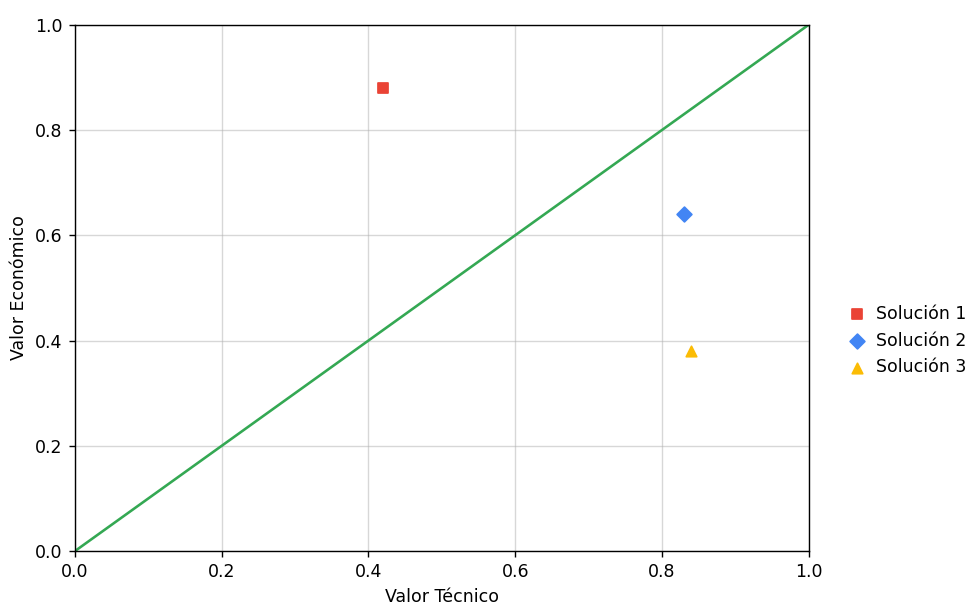
\includegraphics[width=\textwidth]{Imagenes/evtecec.png} \par\medskip
	
	\raggedright
	\footnotesize \textit{Nota.} Elaboración propia.
	\label{fig:EvalTecEc}
\end{figure}


\subsection{Arquitectura de control del concepto óptimo}

\subsubsection{Diagrama de flujo general} 

En la Figura \ref{fig:DiagramaFlujoGeneral}, se detalla la secuencia lógica de arranque y la arquitectura multitarea que gobierna la computadora principal del robot. El proceso inicia con la energización del hardware, donde el sistema operativo inicializa los buses de comunicación y declara una variable global de estado o Flag de Alerta en valor nulo. Posteriormente, el equipo entra en un estado de espera hasta recibir el comando inalámbrico de inicio por parte del operario.

Una vez activado, el software ejecuta una bifurcación propia de arquitecturas orientadas a eventos, dividiendo el procesamiento en hilos paralelos que operan de forma concurrente: un hilo de navegación, un hilo de telemetría y un hilo supervisor de seguridad. En lugar de que cada subproceso gestione sus propias condiciones de parada, los hilos paralelos operan exclusivamente como publicadores de estado. Simultáneamente, el hilo supervisor evalúa la Flag de Alerta de forma continua; si detecta un cambio de estado a valor activo, el supervisor ejecuta una interrupción de máxima prioridad que anula la tracción y transita al sistema hacia un modo seguro.

\begin{figure}[H]
	\captionsetup{justification=raggedright, singlelinecheck=false, labelsep=none}
	
	\caption[Diagrama de flujo de proceso general.]{} 
	
	\textit{Diagrama de flujo de proceso general.} \par\medskip
	
	\centering
	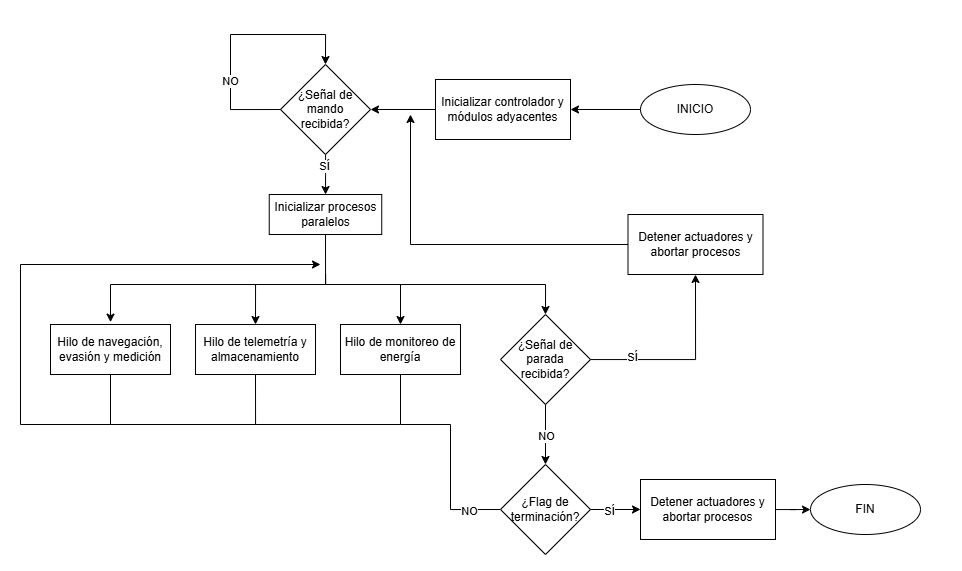
\includegraphics[width=\textwidth]{Imagenes/DiagramaFlujoGeneralTFC1_v2.png} \par\medskip
	
	\raggedright
	\footnotesize \textit{Nota.} Elaboración propia.
	\label{fig:DiagramaFlujoGeneral}
\end{figure}

\subsubsection{Lazo de control del movimiento del robot}

El desplazamiento autónomo del vehículo se rige mediante un lazo de control cerrado en cascada que integra el seguimiento espacial y la regulación de velocidad. Como se observa en la Figura \ref{fig:LazoControl}, la referencia del sistema se calcula dinámicamente comparando la ruta predefinida con las coordenadas espaciales retroalimentadas por la antena GPS de parche cerámico y la orientación provista por la unidad IMU. Esta fusión de datos alimenta al algoritmo geométrico Pure Pursuit, el cual calcula el error de desvío lateral para definir el ángulo de corrección requerido.

De forma paralela, la retroalimentación de los encoders rotativos determina el error respecto a la velocidad nominal operativa de 1 m/s. El controlador central, mediante un algoritmo PID, amalgama ambos errores para generar y distribuir las señales de Modulación por Ancho de Pulsos hacia los actuadores. Al tratarse de un chasis de tracción diferencial, el PID varía la potencia entre los flancos izquierdo y derecho para corregir el rumbo y mantener al robot sobre la trayectoria ideal sin interrumpir su avance.

\begin{figure}[H]
	\captionsetup{justification=raggedright, singlelinecheck=false, labelsep=none}
	
	\caption[Lazo de control del movimiento de traslación del robot.]{} 
	
	\textit{Lazo de control del movimiento de traslación del robot.} \par\medskip
	
	\centering
	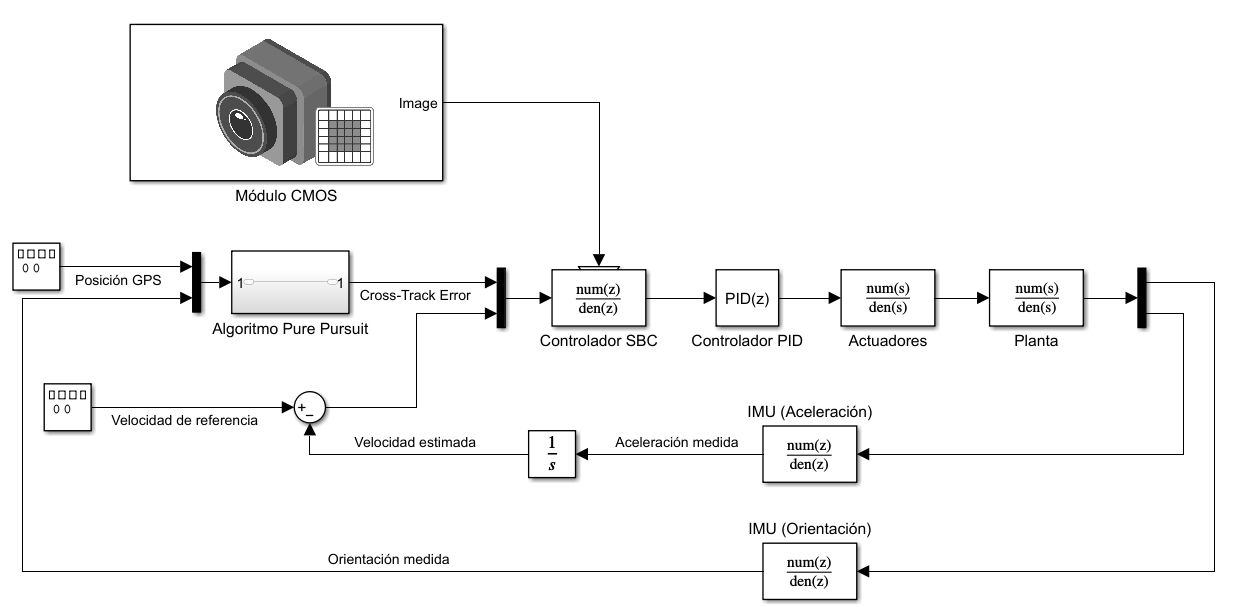
\includegraphics[width=\textwidth]{Imagenes/LazoControlSolucionOptima.png} \par\medskip
	
	\raggedright
	\footnotesize \textit{Nota.} Elaboración propia.
	\label{fig:LazoControl}
\end{figure}

\subsubsection{Topología de red}

La arquitectura de comunicaciones, vista en la Figura \ref{fig:TopologiaRed}, del sistema emplea una topología punto a punto fundamentada en el protocolo de radiofrecuencia LoRa. En este esquema, el robot de inspección actúa como un nodo terminal móvil equipado con un módulo transceptor LoRa que concentra los datos meteorológicos procesados.

La capa de red establece un enlace bidireccional de baja potencia y largo alcance con la estación base o Gateway ubicada en las instalaciones del parque fotovoltaico, garantizando una cobertura efectiva superior a los 200 metros. El enlace de subida se encarga de transmitir los paquetes de telemetría y alertas de obstáculos hacia el servidor central para su visualización y almacenamiento, mientras que el enlace de bajada permite que el dispositivo escuche continuamente comandos del exterior, posibilitando la recepción de instrucciones críticas como el telecomando de parada remota emitido por el operario.

\begin{figure}[H]
	\captionsetup{justification=raggedright, singlelinecheck=false, labelsep=none}
	
	\caption[Topología de red con los robots como nodos.]{} 
	
	\textit{Topología de red con los robots como nodos.} \par\medskip
	
	\centering
	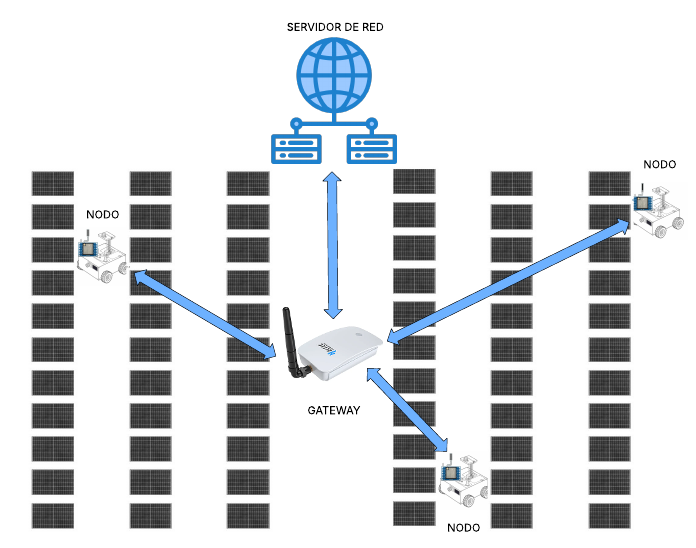
\includegraphics[width=\textwidth]{Imagenes/TopologiaRedTFC1.png} \par\medskip
	
	\raggedright
	\footnotesize \textit{Nota.} Elaboración propia.
	\label{fig:TopologiaRed}
\end{figure}


%%%%
\subsection{Arquitectura electrónica del concepto óptimo}

\subsubsection{Diagrama de bloques} 

La Figura \ref{fig:DiagramaBloques}, ilustra la integración de hardware del concepto de solución seleccionado, segmentada según las interfaces de potencia y datos. La matriz energética está constituida por un paquete de baterías Li-Ion gestionado por un sistema BMS, el cual fluye a través de fusibles electrónicos que otorgan protección activa contra cortocircuitos. Desde este punto, la energía se bifurca hacia convertidores Buck DC-DC y reguladores lineales que independizan y estabilizan los niveles de tensión para aislar el ruido eléctrico entre la electrónica de control y la carga inductiva de los actuadores.

En el nivel de procesamiento, la Placa SBC actúa como el nodo maestro. A través de sus buses de datos digitales, consolida la conexión con los dispositivos periféricos: la antena GPS, la unidad IMU, la memoria MicroSD y el módulo de comunicaciones LoRa. Paralelamente, adquiere las lecturas analógico-digitales de la cámara CMOS frontal y los sensores meteorológicos. Finalmente, los pines de salida del microprocesador comandan los drivers de potencia que accionan los motores de tracción DC y los servomotores responsables de la cinemática de la plataforma de instrumentación.

\begin{figure}[H]
	\captionsetup{justification=raggedright, singlelinecheck=false, labelsep=none}
	
	\caption[Diagrama de bloques representativo de la arquitectura eléctrica.]{} 
	
	\textit{Diagrama de bloques representativo de la arquitectura eléctrica.} \par\medskip
	
	\centering
	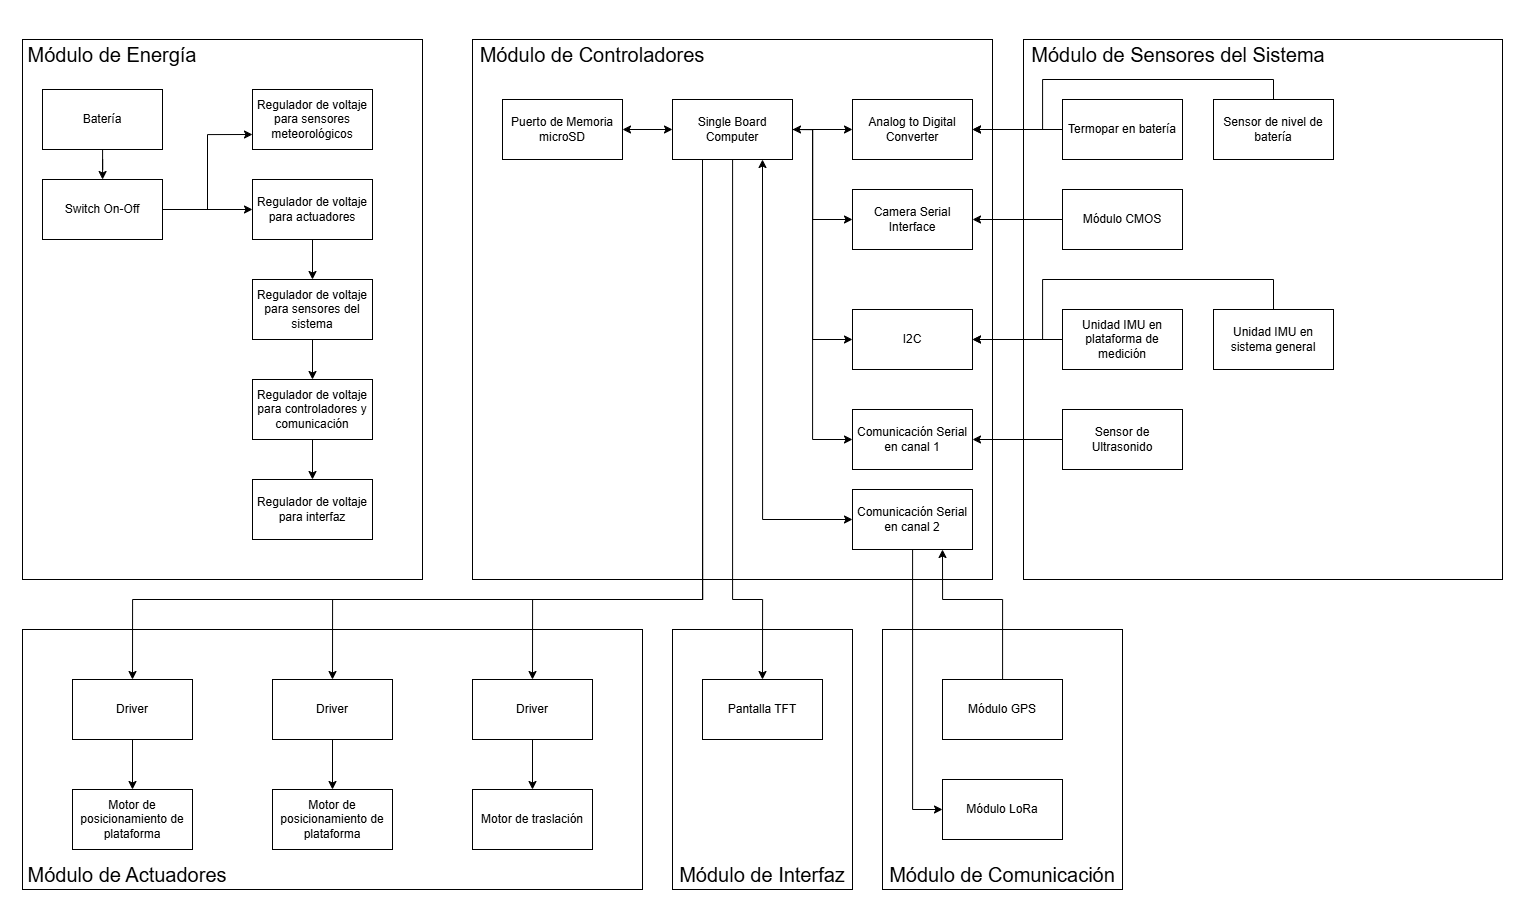
\includegraphics[width=\textwidth]{Imagenes/DiagramaBloquesTFC1_v2.png} \par\medskip
	
	\raggedright
	\footnotesize \textit{Nota.} Elaboración propia.
	\label{fig:DiagramaBloques}
\end{figure}
%%%%%
\subsection{Vista general del concepto óptimo}


\begin{figure}[H]
	% Fuerza la alineación izquierda y quita los ":" después del número
	\captionsetup{justification=raggedright, singlelinecheck=false, labelsep=none}
	
	\caption[Vista general del concepto óptimo.]{} 
	
	% Vspace negativo opcional para acercar el texto cursivo al número de figura
	\textit{Vista general del concepto óptimo.} \par\medskip
	
	\centering
	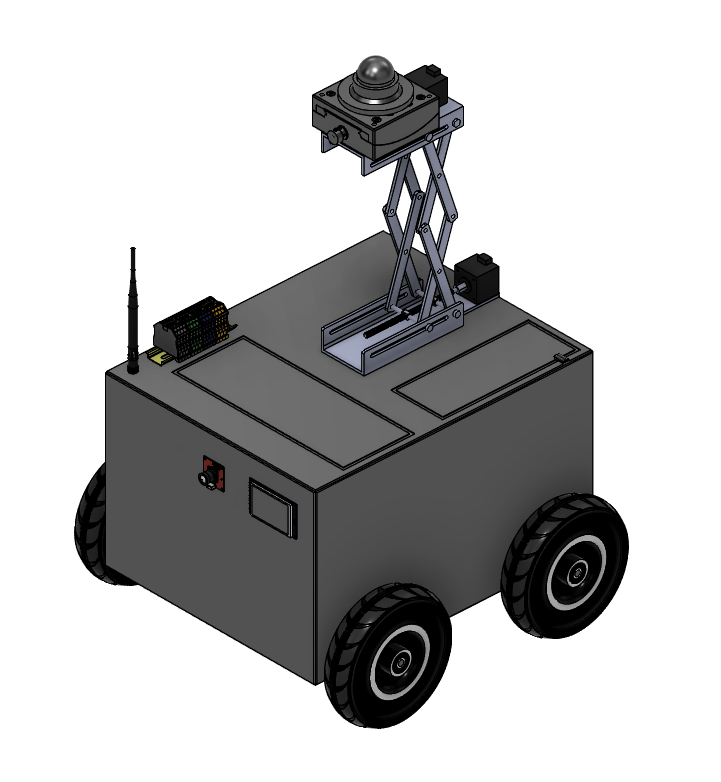
\includegraphics[width=0.6\textwidth]{Imagenes/CAD-GENERAL_V1.png} \par\medskip
	
	\raggedright
	\footnotesize \textit{Nota.} Elaboración propia.
	\label{fig:CADGENERAL}
\end{figure}

\subsection{Subsistemas mecánicos del concepto óptimo}

\subsubsection{Subsistema de traslación}

	\begin{figure}[H]
	
	\captionsetup{justification=raggedright, singlelinecheck=false, labelsep=none}
	
	\caption[Vista isometrica y frontal del subsistema de traslación.]{} 
	
	\textit{Vista isometrica y frontal del subsistema de traslación.} \par\medskip
	
	\begin{minipage}{0.5\textwidth}
		\centering
		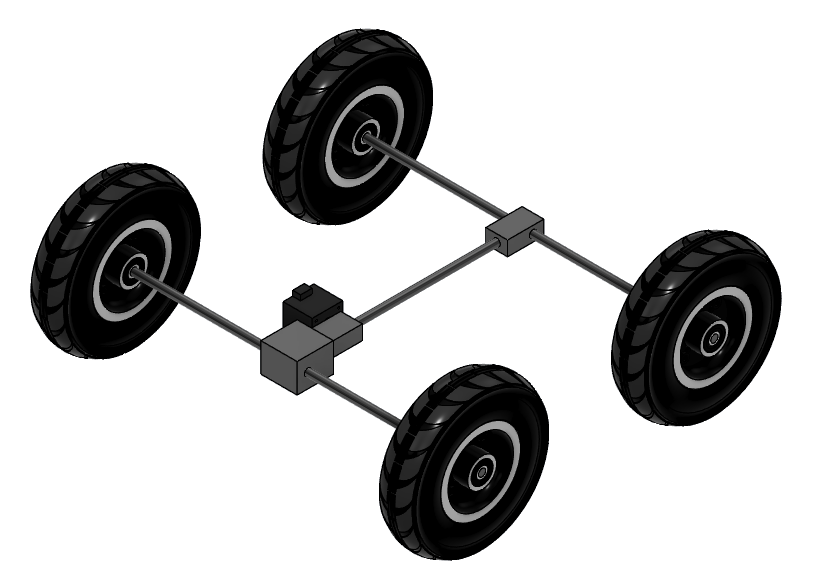
\includegraphics[width=\linewidth]{Imagenes/SISTEMA_TRASLACION_ISO.png}
	\end{minipage}\hfill
	\begin{minipage}{0.5\textwidth}
		\centering
		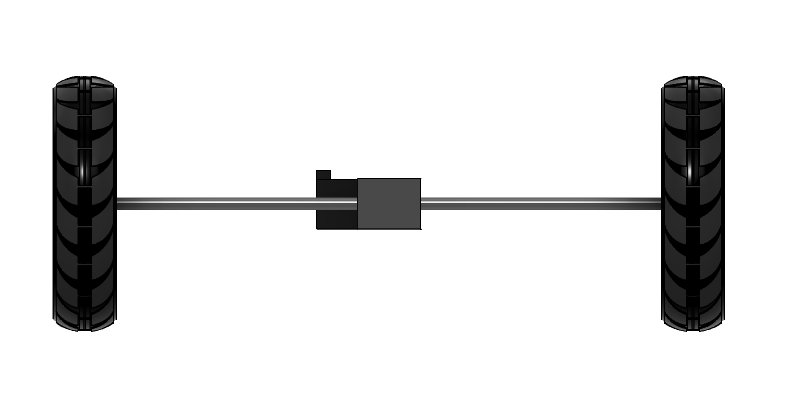
\includegraphics[width=\linewidth]{Imagenes/SISTEMA_TRASLACION_FRONT.png}
	\end{minipage}
	\par\medskip
	
	\raggedright
	\footnotesize \textit{Nota.} Elaboración propia.
	\label{fig:SubsistemaTraslacion}
\end{figure}


\subsubsection{Subsistema de posicionamiento de plataforma de medición}


\begin{figure}[H]
	
	\captionsetup{justification=raggedright, singlelinecheck=false, labelsep=none}
	
	\caption[Vista isometrica y derecha del subsistema de posicionamiento.]{} 
	
	\textit{Vista isometrica y derecha del subsistema de posicionamiento.} \par\medskip
	
	\begin{minipage}{0.5\textwidth}
		\centering
		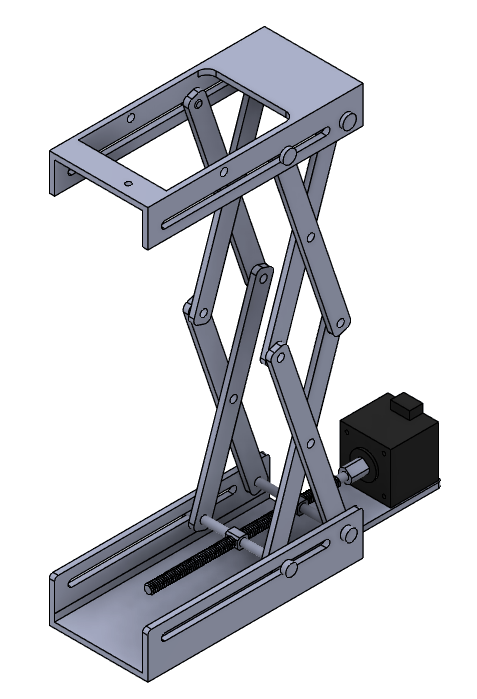
\includegraphics[width=\linewidth]{Imagenes/MECANISMO_POSICION_ISO.png}
	\end{minipage}\hfill
	\begin{minipage}{0.5\textwidth}
		\centering
		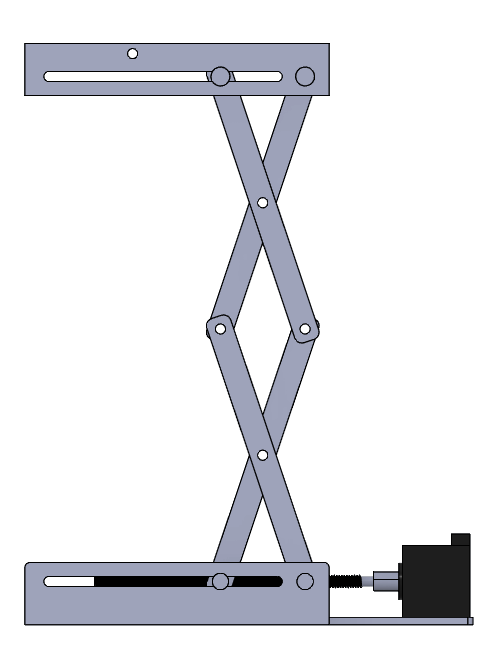
\includegraphics[width=\linewidth]{Imagenes/MECANISMO_POSICION_DERECHA.png}
	\end{minipage}
	\par\medskip
	
	\raggedright
	\footnotesize \textit{Nota.} Elaboración propia.
	\label{fig:SubsistemaPosicionamiento}
\end{figure}


\subsubsection{Subsistema de orientación de plataforma de medición}


\begin{figure}[H]
	
	\captionsetup{justification=raggedright, singlelinecheck=false, labelsep=none}
	
	\caption[Vista isometrica y derecha del subsistema de orientación.]{} 
	
	\textit{Vista isometrica y derecha del subsistema de orientación.} \par\medskip
	
	\begin{minipage}{0.5\textwidth}
		\centering
		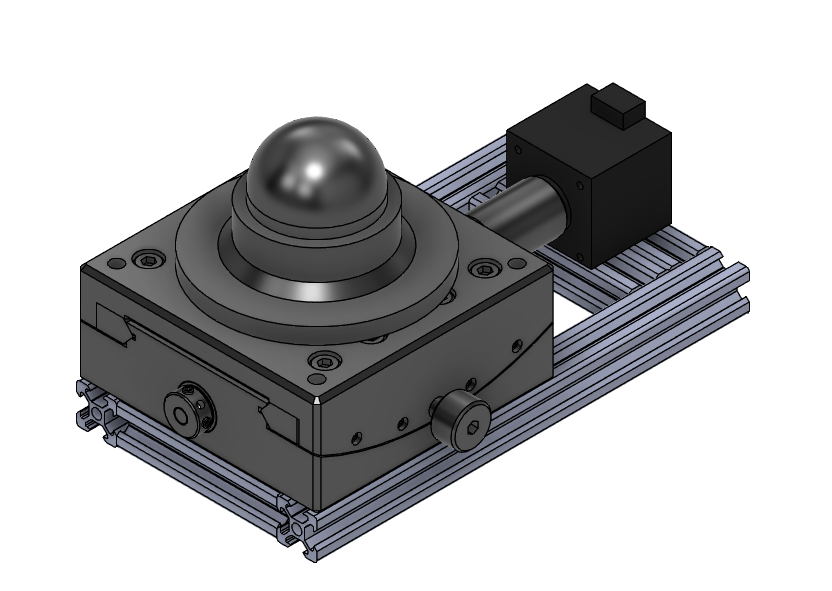
\includegraphics[width=\linewidth]{Imagenes/MECANISMO-ORIENTACION-ISO.png}
	\end{minipage}\hfill
	\begin{minipage}{0.5\textwidth}
		\centering
		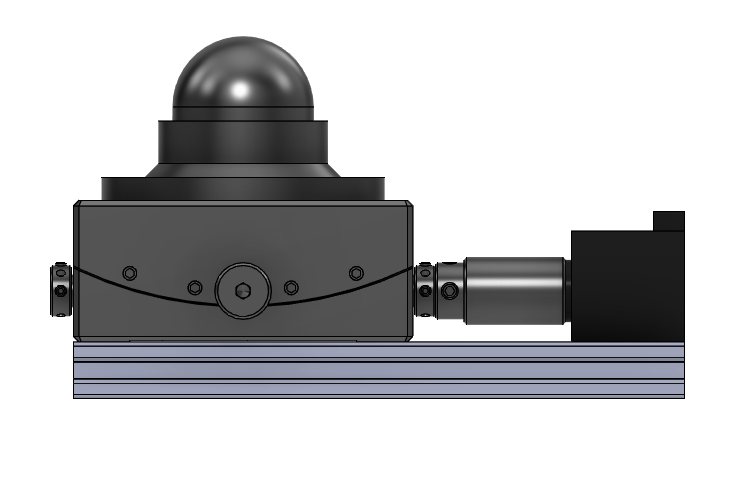
\includegraphics[width=\linewidth]{Imagenes/MECANISMO-ORIENTACION-DERECHA.png}
	\end{minipage}
	\par\medskip
	
	\raggedright
	\footnotesize \textit{Nota.} Elaboración propia.
	\label{fig:SubsistemaOrientacion}
\end{figure}

\subsubsection{Estructura de soporte}

\begin{figure}[H]
	% Fuerza la alineación izquierda y quita los ":" después del número
	\captionsetup{justification=raggedright, singlelinecheck=false, labelsep=none}
	
	\caption[Vista isométrica de la estructura.]{} 
	
	% Vspace negativo opcional para acercar el texto cursivo al número de figura
	\textit{Vista isométrica de la estructura.} \par\medskip
	
	\centering
	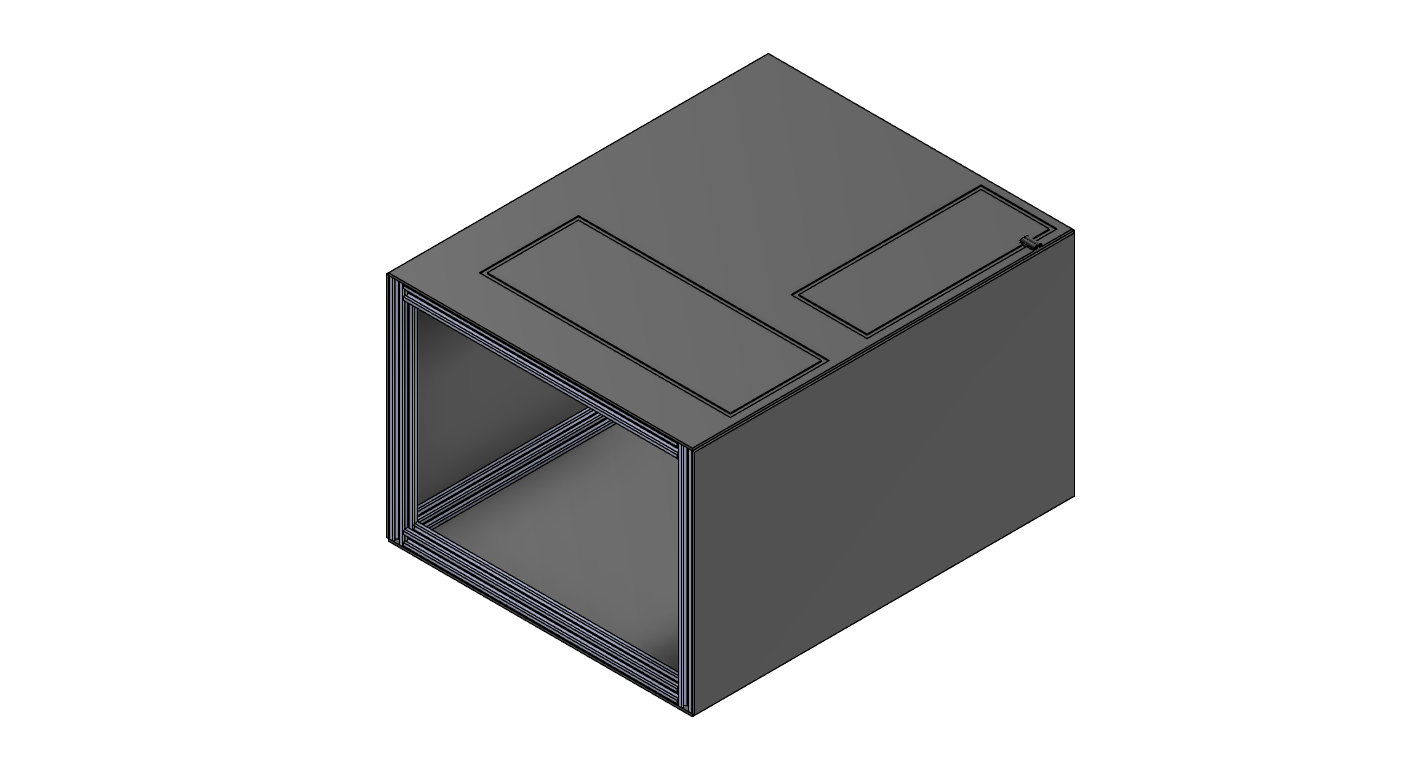
\includegraphics[width=\textwidth]{Imagenes/SOPORTE-CUBIERTA-ISO.png} \par\medskip
	
	\raggedright
	\footnotesize \textit{Nota.} Elaboración propia.
	\label{fig:CarcasaISO}
\end{figure}






